\pdfoutput=1
\documentclass[11pt]{article}

\usepackage{graphicx}
\usepackage[space]{grffile}
\usepackage{latexsym}
\usepackage{textcomp}
\usepackage{longtable}
\usepackage{multirow,booktabs}
\usepackage{amsfonts,amsmath,amssymb}
\usepackage{url}
\usepackage{hyperref}
\hypersetup{colorlinks=false,pdfborder={0 0 0}}
% You can conditionalize code for latexml or normal latex using this.
\newif\iflatexml\latexmlfalse
\usepackage[utf8]{inputenc}
\usepackage[english]{babel}

\usepackage{setspace}
\usepackage{apacite}
\usepackage[margin=1in]{geometry}



\begin{document}

\title{Analysis of Dyadic Interaction in an Job Interview Setting}

\author{Suresh Alse, Bhavishya Sharma, Jay Priyadarshi, Abhishek Sharma}

\maketitle




\nocite{*}
\section{Introduction}
Interviews are often hard to be judged. It is often left in the hands of the interviewer(s) to measure the hirability of the candidates. This is fundamentally flawed as this heavily relies of interviewers' mood and personality. Also, in most cases multiple interviewers interview for the same roles which makes this process even less scientific as it is almost impossible to fairly aggregate the opinions of interviewers.

There has been tons of research by psychologists and career experts about what one should do in order to succeed in an interview \cite{huffcutt2001identification}. From this, we know that things like smiling, using a confident tone and making good eye contact can contribute a lot in an interview. However, these observations are often based on intuition and experience. Hence, It is hard to automate and quantify hirability of candidates. Also, there is a common misconception that content of the interviewee's responses is the sole determinant of the job interview. However, it is seen that non verbal aspects are as important if not more important than verbal responses \cite{mehrabian1971silent}.

\begin{figure}[h!]
\begin{center}
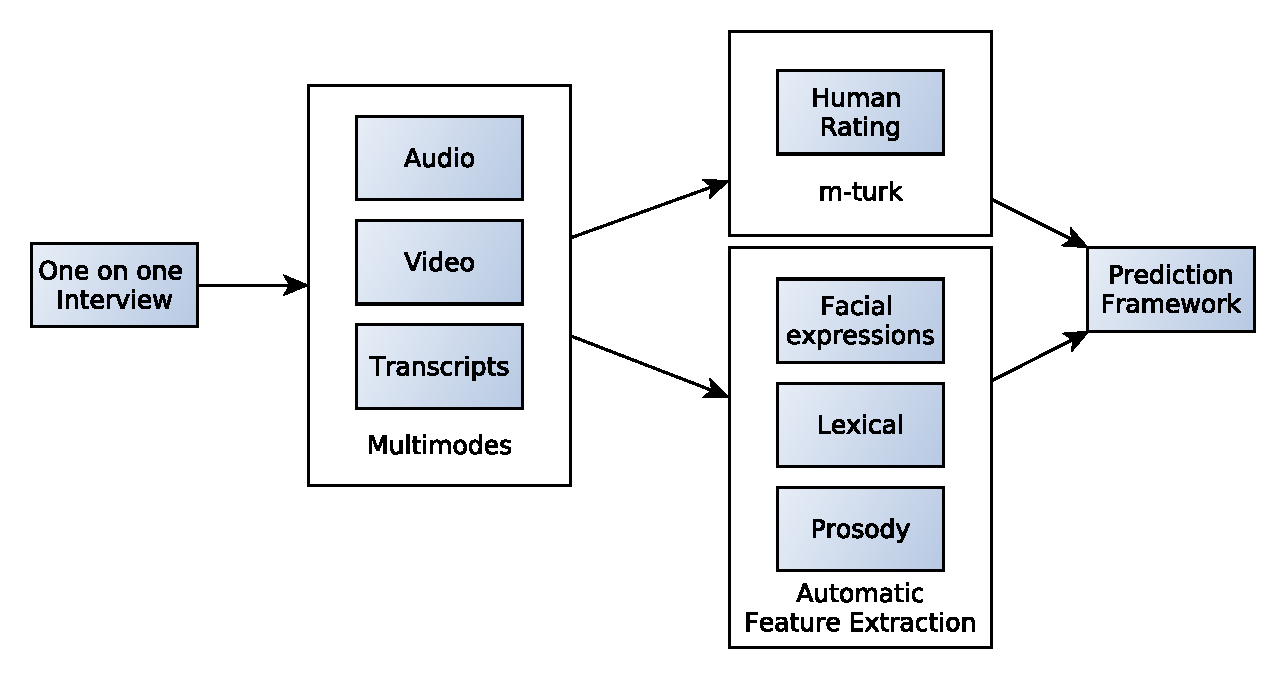
\includegraphics[width=0.7\columnwidth]{figures/process1/process1}
\label{fig:process}
\caption{{Proposed Framework%
}}
\end{center}
\end{figure}

In this project we would like to build a computational framework using which interviewers and interviewees can use it to analyze interviews and obtain the following.
\begin{itemize}
\item Automatically predict the overall score of the interview.
\item Quantify verbal and nonverbal behavior of the interviewee towards the success in the interview.
\item Automatically recommend aspects to be improved for better overall score. 
\item Timeline that shows how well the interview progressed with respect to each question.
\end{itemize}

In order to achieve this we propose a framework as shown in Figure \ref{fig:process}. We use a one on one interview data comprised of three modes (audio, video and textual). Then, we extract multimodal features (facial expressions, lexical and prosody) and predict the overall score of the interview, how likely the candidate is going to be hired and other traits required for the interview process.


\section{Related Work}
A lot of the research in the field of mulitmodal analysis of interaction has focused on speech and visual analysis of data. For instance, in Rough'n'Ready: A Meeting Recorder and Browser \cite{kubala1999rough}, they provide a way to recognize speech in the form of a BBN Byblos Speech Recognition System, where they also provide a mechanism to browse and retrieve speech data with the help of a speech index. Speaker identification is also described in The Meeting Project at ICSI \cite{morgan2001meeting}, where the acoustic model consisted of gender-dependent, bottom-up clustered (genonic) Gaussian mixtures. Further, leveraging speech recognition, topic detection in a meeting room scenario is described in Advances in Automatic Meeting Record Creation and Access, where they use a variant of Hearst's TextTiling algorithm in order to automaticaly segment the transcript into topically coherent passages.

As far as visual analysis is concerned, we can find examples of that in SMaRT: The Smart Meeting Room Task at ISL \cite{waibel2003smart}, where they provide a mechanism to track people and identify them as they move around a Meeting Room using multiple cameras and advanced computer vision techniques. Another good example of that would be Distributed Meetings: A Meeting Capture and Broadcasting System \cite{cutler2002distributed} where they augment the meeting room for remote viewers by adding cameras and other functionalities.

A major focus on such speech and visual processing (as provided above) has been focused on individuals, however, even when the researchers examine a meeting space. Our aim is to analyze dyadic communication where we don't just monitor an individual, but we attempt to find multimodal cues (such as back-channels among others) which would then uncover the underlying mechanism of a job interview.

There has been research on analyzing behavior of a group as compared to an individual, as is exemplified by research like The KidsRoom: A Perceptually-Based Interactive \cite{bobick1999kidsroom} and Immersive Story Environment and A Bayesian Computer Vision System for Modeling Human Interactions \cite{oliver2000bayesian}. However, the research here focuses on problem specific "primitive tasks", and therefore involves a much more constrained examination, which is in a sharp contrast to a sort of free-flowing, spontaneous (dyadic) interaction that we would have hoped for.

While our system focuses on some form of speech and visual processing, and also incorporates analysis of dyadic interaction as a whole, we provide a way to analyze the interaction in a much more unconstrained manner, identifying key multimodal cues, unraveling the underlying operating factors of a job interview by treating an interview as "more than a some of its parts" and hopefully, to come up with capabilities to automatically predict the overall score of an interview, quantify verbal and non verbal behavior of the interviewee towards the success in the interview, automatically recommend aspects to be improved for a better overall score, and a timeline to show how well an interview progressed with respect to time.

\section{Dataset}
We use the MIT Interview Dataset \cite{naim2015automated} for this project that we obtained by contacting the authors of the project. It consists of 138 recordings of mock interviews of students from MIT, seeking internships. The interviews were conducted in a one on one interview fashion. Both interviewers and interviewees were equipped with microphones which allows us to extract and differentiate between the speakers easily. Cameras were used to capture the video of the interviewee during the process as shown in the Figure \ref{fig:dataset}. The interviews were conducted by two professional career counselors with over five years of interviewing experience. All participants are native english speakers (this is very important because in our approach things like confidence, fluency, etc are considered). For every participant, two rounds were conducted - before and after intervention. Overall, 69 students permitted the use of recordings for research purposes. Hence we have a total of 138 recordings of lengths between 3 minutes to 8 minutes (average: 4.7 minutes per interview). Every interview consisted of interviewer asking the interviewee, five questions and no job description was given to the interviewees. The researchers who collected this data claim that this is the largest collection of job interview videos conductedby professionals.

To rate the interview, Amazon mechanical turk workers were used. Each turker watched the interview videos and rated the interviews by answering 16 assessment questions \ref{tab:assess} on seven point scale. Questions about ``Overall rating'' and ``Recommend Hiring'' captures overall score where as other questions capture higher level behavior. 
\begin{table}[h!]
    \centering
    \begin{tabular}{ | c | }
	\hline
        Engagement \\
	\hline
        Excited \\
        \hline
        Friendly \\
        \hline
        Smiled \\
        \hline
        NoFillers\\
        \hline
        RecommendedHiring \\
        \hline
        Overall \\
        \hline
        EyeContact\\
        \hline
        NotAwkward\\
        \hline
        StructuredAnswers\\
        \hline
        Calm \\
        \hline
        Focused\\
        \hline
        NotStressed\\
        \hline
        Authentic\\
        \hline
        Paused \\
        \hline
        SpeakingRate\\
        \hline
    \end{tabular} 
    \caption{Assessment questions}
    \label{tab:assess}
\end{table}

The dataset also consists of transcripts of all the interviews. This was made possible by Amazon mechanical turk workers hired by the researchers. Also, they were instructed to include filler words such as ``like'', ``uh'', ``umm'' along with cues like ``[long pause]'', ``[smiling]'' etc which are very useful for our process.

We also tried semaine-db \cite{mckeown2012semaine} which seemed good for this project. However, it just consisted data of two individuals talking to each other and was in no way an interview setting. We also considered using AMI database which consisted of a group discussing about a particular topic for a day. However, this had additional problems such as multiple people in a frame, etc and moreover similar to semaine-db, this was not a interview setting. Also, as this needs a considerable amount of data in a given setting and then requires amazon mechanical turkers, creating our own dataset seemed farfetched. Hence, we chose MIT Interview Dataset which is perfect for our project. 

\begin{figure}[h!]
\begin{center}
\includegraphics[width=0.7\columnwidth]{figures/Screenshot from 2016-10-21 20-30-05/Screenshot from 2016-10-21 20-30-05}
\caption{One of the 138 interviews.}
\label{fig:dataset}
\end{center}
\end{figure}

\subsection{Drawbacks}
\begin{itemize}
 \item As the study is limited to undergraduate students, it might have introduced a selection bias in the dataset. 
 \item In the dataset, there are occasions where a small mistake (like using a swear word) would reflect badly on the interview outcome. As they are very rare, it is difficult to model such phenomena.
 \item The dataset has a set of 138 interviews, in which 69 interviews are before feedback is shared, while 69 are with the same participants, after the feedback is shared. This provides a bit of redundancy to an already biased dataset. As of now, we are treating each interview distinctly, however it is still up for discussion.
 \item In the dataset, the interviewer is not visible, and hence we are not able to model the interviewer’s nonverbal behavior.
\end{itemize}

\subsection{Inter-rater agreement}
To gauge the quality of the ratings given by 9 annotators, we have calculated Krippendorff’s Alpha for each trait. The ratings are on a 7-point scale. Figure \ref{fig:interrater} shows that the annotators agreed more on the if the subject had an Engaging tone, if they seemed Excited, Friendly or smiled. This can be because of the fact that we have developed necessary insticts to easily notice these things and we would almost always agree with features like if a individual smiled or if he/she was friendly or excited or even had an engaging tone. Whereas the features like Structured Answer, Authentic, Calm, paused, Speaking rate are kind of features which a lot of humans would disagree on: An idea can be Authentic to one individual might not feel Authentic to another. The same thing, measuring the Structure of an answer, Calmness, Speaking rate and Focus of an individual is something which will incur a high variance among annotators. Different annonators may have diffferent criteria for deciding the structure of an answer. Hence, it can be seen that traits like Engaging Tone, Excited, Friendly, No Fillers, Smile have good inter-annoatator agreement, where as in case of subjective traits like Structured Answer, Authentic, Stress, etc. get low scores.

\begin{figure}[h!]
\begin{center}
\includegraphics[width=1\columnwidth]{figures/k-alpha scores.png}
\caption{Krippendorff's Alpha}
\label{fig:interrater}
\end{center}
\end{figure}

\subsection{Feature analysis}
\label{sec:feature_analysis}
We extract Prosodic, Facial and Lexical features from the dataset as mentioned in Section \ref{sec:methodology}. Also, we did some analysis on the features extracted to get more insights to do feature selection while doing regression. For every feature we try to find the correlation between the features and the scores of assessment questions.
\subsubsection{Prosodic Features}
The extracted prosodic features consists of energy, power, pitch etc. Every interview is divided into five segments corresponding to five different questions asked by the interviewer. After averaging out all the features for each of the segments, we try to match it with the scores assigned by the turkers for each of the assessment questions. We draw a scatter plot and try to fit a line to see how relevant the score is to each of these features. A positive slope indicates that with the increase in the value of the feature, a higher score would be assigned. A negative slope would indicate that with the increase in the value of the feature, a lower score would be assigned. A near zero slope would indicate that this feature wouldn't matter and we can neglect it in regression. Figures \ref{fig:prosodic_analysis1}, \ref{fig:prosodic_analysis2}, \ref{fig:prosodic_analysis3} and \ref{fig:prosodic_analysis4} are some of the 1026 graphs that were drawn to visualize this. In Figure \ref{fig:prosodic_analysis1} we can see that with the increase in energy, interviewees are likely to be more excited. Figure \ref{fig:prosodic_analysis2} indicates that the recommended rating score drops with the increase in shimmer. Figure \ref{fig:prosodic_analysis4} indicates that Min pitch and Engaged score are not related and hence we can ignore it. 

\begin{figure}[h!]
\begin{center}
\includegraphics[width=0.65\columnwidth]{figures/Excited and energy.png}
\caption{Energy vs Excited}
\label{fig:prosodic_analysis1}
\end{center}
\end{figure}

\begin{figure}[h!]
\begin{center}
\includegraphics[width=0.65\columnwidth]{figures/RecommendHiring and shimmer.png}
\caption{Shimmer vs Recommended Hiring}
\label{fig:prosodic_analysis2}
\end{center}
\end{figure}

\begin{figure}[h!]
\begin{center}
\includegraphics[width=0.65\columnwidth]{figures/NotAwkward and energy.png}
\caption{Energy vs NotAwkward}
\label{fig:prosodic_analysis3}
\end{center}
\end{figure}

\begin{figure}[h!]
\begin{center}
\includegraphics[width=0.65\columnwidth]{figures/NoFillers and energy.png}
\caption{Energy vs No. of Fillers}
\label{fig:prosodic_analysis3}
\end{center}
\end{figure}


\begin{figure}[h!]
\begin{center}
\includegraphics[width=0.65\columnwidth]{figures/Engaged and min_pitch.png}
\caption{Min Pitch vs Engaged}
\label{fig:prosodic_analysis4}
\end{center}
\end{figure}

As we observe direct correlation between these extracted features, we can consider these directly in our approach.

\subsubsection{Facial Features}
Facial features extracted are composed of features such as pitch, yaw, roll etc of the face at every frame. By taking average of the features of the frames corresponding to every question we do similar analysis as we did in case of prosodic features. Figure \ref{fig:facial_analysis} shows how pitch of the face varies with engaged.

\begin{figure}[h!]
\begin{center}
\includegraphics[width=0.65\columnwidth]{figures/Engaged and Pitch.png}
\caption{Pitch vs Engaged}
\label{fig:facial_analysis}
\end{center}
\end{figure}

We see that this approach doesn't give much insights about the assessment questions. So, we can't just use these features and we have to do some feature extraction from these features which we describe in Section \ref{sec:methodology}.

\section{Methodology}
\label{sec:methodology}
This section we describe the overall approach towards building the proposed framework.

\subsection{Feature Extraction}
We consider three categories of features in our approach i.e Prosodic features, lexical features and facial features. Also, as the data provides with necessary transcripts from m-turkers along with filler words, we don't have to use any automatic speech recognition. Hence lexical features can be extracted directly from transcripts.
\subsubsection{Prosodic Features}
In order to extract prosodic features from the audio, we used an open source speech analysis tool called PRAAT \cite{naim2015automated}. From the dataset we know the durations of each of the question asked during the interview. So each interview can be divided into five parts. We extract prosodic features over these five parts and keep it separately.

According to some of the previous research \cite{frick1985communicating}, pitch, intensity, characters of first three formants and spectral energy are found to be more representative of our behavior. For every feature we extracted mean, variance, minimum and maximum values. We also extracted additional features such as pauses, non-uniform pitch and intensity of speeches as it will help in determining overall score of the interview.
\subsubsection{Lexical Features}
Word count is often used as lexical feature in many applications. However, we only have limited data; hence, we will not be able to use it as it would result in sparse high dimentional feature vectors. To resolve this problem, we will use Latent Dirichlet Allocation (LDA) to learn 20 topics from interview dataset. Then, we use the relative weights of these topics in every interview as lexical features.

Also, we know that speaking rate and fluency can be indicators of a good interview. Hence, we are also planning to use additional features such as words per second, unique words per second, filler word count and unique word count. 
\subsubsection{Facial Features}
Facial features are very important and are hard to be quantified. In this project, we extract features from every frame in the video sequence. The dataset includes the facial features extracted for each video using Shore framework. We will divide every video into five parts corresponding to the questions asked. Using AdaBoost classifier to distinguish between neutral and smiling faces, the dataset also gives us the smile data that we can use. We will extract things such as head nods and shakes and average it out and consider as a feature. 

We will normalize all the features to have zero mean and unit variance to eliminate bias.

\subsection{Score Predictions}
We use the features extracted as mentioned above to predict the final score.
\subsubsection{Training}
Figure \ref{fig:methodology-training} shows the overall approach for training. We treat aggregate of every assessment question scored by the turkers as a feature and concatenate them to form a feature vector. The overall score rounded to nearest score in the 1-7 point scale is considered as the training class. We use the feature vector and the the score to train a SVM model which can be used to predict scores.
\begin{figure}[h!]
\begin{center}
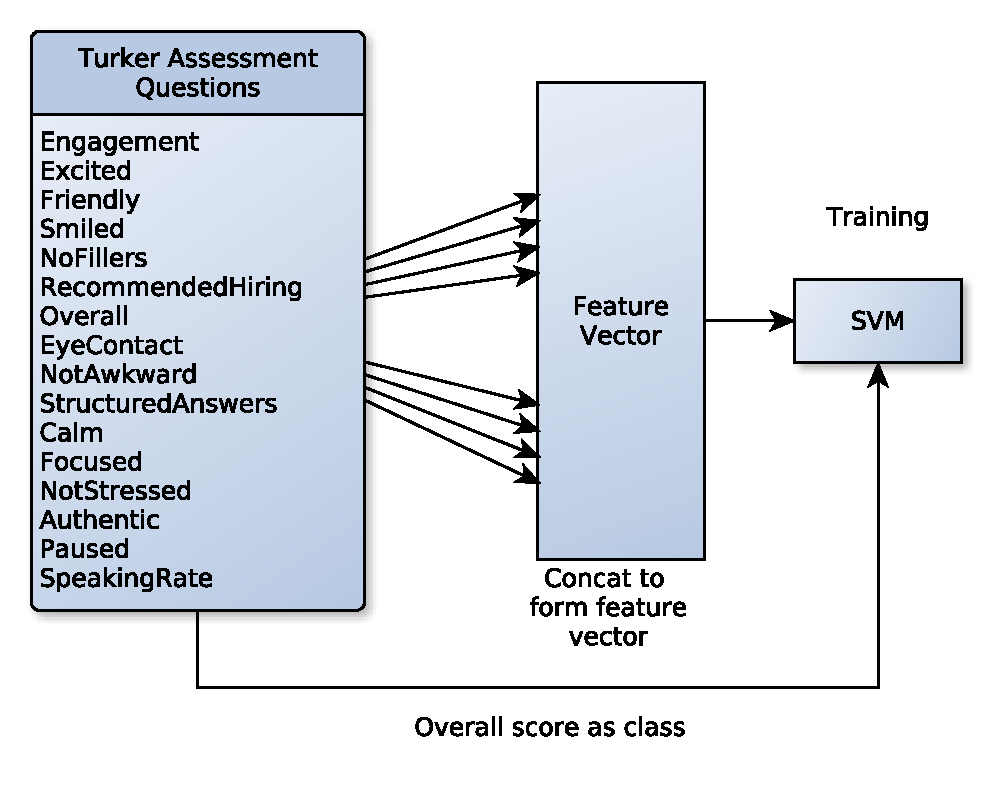
\includegraphics[width=0.7\columnwidth]{figures/methodology-training.pdf}
\caption{Training}
\label{fig:methodology-training}
\end{center}
\end{figure}
\subsubsection{Classification}
After training the SVM model we will use it as mentioned in the Figure \ref{fig:methodology} for prediction. After extracting the multimodal features, we will perform feature selection as mentioned in Section \ref{sec:feature_analysis} to select appropriate features for each of the assessment questions. We will use SVR type of regression to predict the scores for assessment questions. Assessment scores used to train the SVM model is used to train SVR as well. While predicting the scores of assessment questions, we do it on question level i.e every question asked by the interviewer. Once, we have the assessment question scores, we concatenate it to form a feature vector. This is then passed to SVM classifier trained earlier to predict the final score. For every interviewee, we will have five results corresponding to each question. The average score is considered to see if the interviewee should be hired or not.

\begin{figure}[h!]
\begin{center}
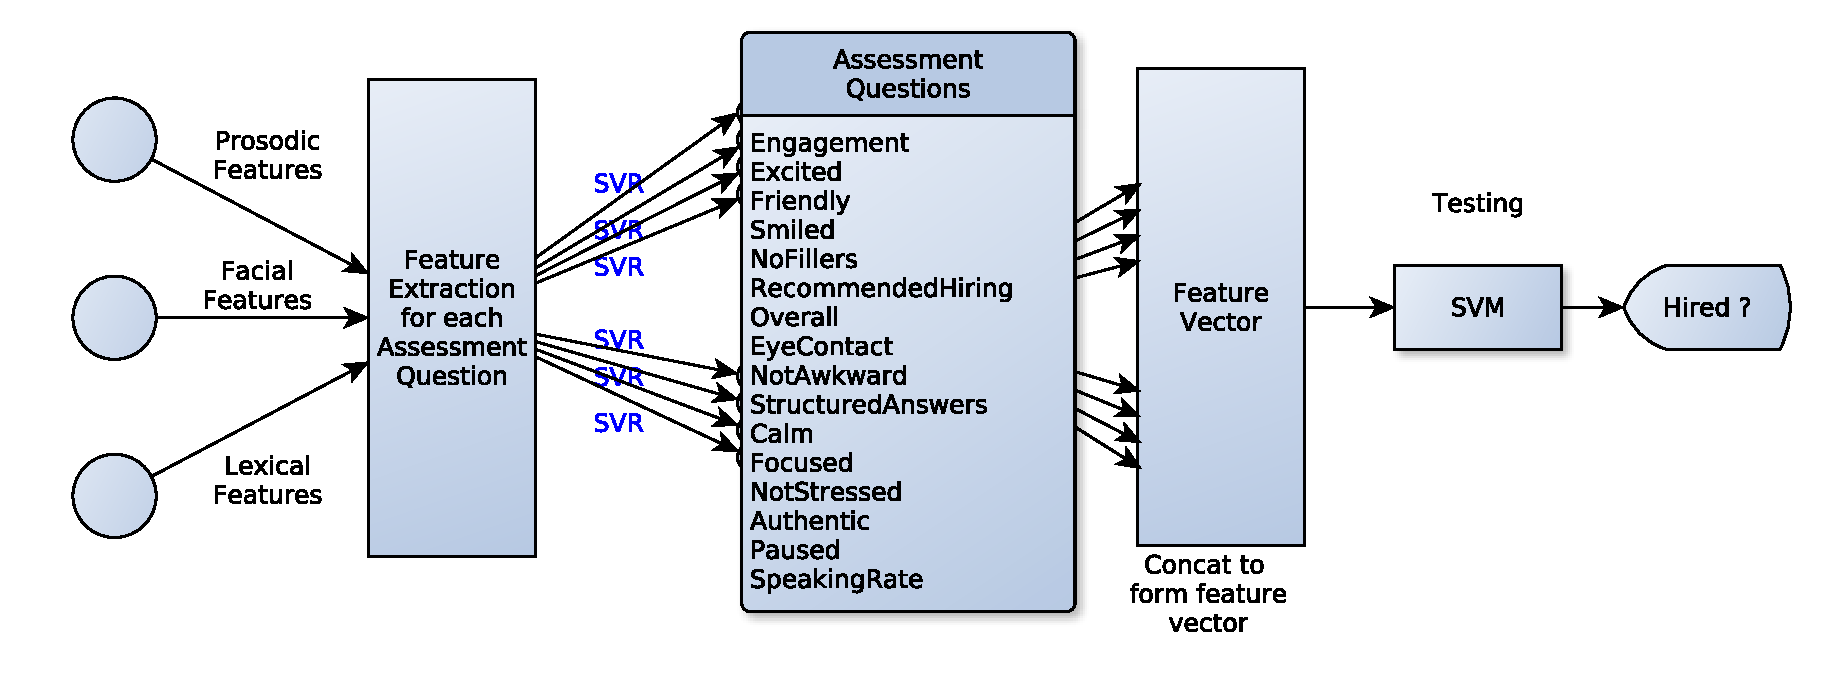
\includegraphics[width=1\columnwidth]{figures/methodology.pdf}
\caption{Prediction}
\label{fig:methodology}
\end{center}
\end{figure}

\subsubsection{Score analysis and Report generation}
SVM classifier also allows us to find the weights of the feature vectors while doing the prediction. Using this, we can measure things like engagement, how excited, how friendly. etc (from assessment questions) the interviewee was in the interview. As we have done this on the question level (five questions per interview), we can go to the level to which we will be able to tell specific parts where the interviewee excelled or needs improvement.

\subsubsection{Validation}
\begin{figure}[h!]
\begin{center}
\includegraphics[width=0.6\columnwidth]{figures/validation.jpeg}
\caption{Validation}
\label{fig:methodology}
\end{center}
\end{figure}
All the experiments mentioned above are run in a leave-one-interview-out fashion, i.e. we keep the examples in the testing set (25\%) segregated from the training (50\%) and validation sets (25\%). The criteria for inclusion of a certain interview in any of the datasets is random (although, we need to make sure that the pre and post pairs don’t end up in the same dataset). The optimal model parameters for each test set are chosen by a three–fold validation on the remaining interviews, with the evaluation metric used being total accuracy, i.e. percentage of interviews for which correct label is predicted in a test set.

\section{Timeline}
\begin{table}[h!]
    \begin{tabular}{ | c | p{13cm} | }
	\hline
        Mid Term & Prosodic, lexical and facial feature extraction. \newline Aggregating the features to form feature vectors of all required types. \newline \\
	\hline
        Post Mid Term &  Use evaluation techniques for feature extractions. \newline Develop a plug and play like system to test out different approaches of regression.\newline \\ 
        \hline
        Final & Use SVC and Lasso to estimate scores of the interviews and find accuracy of our approach. \newline Build a system that can generate reports, graphs and recommendations.\newline \\ 
        \hline
    \end{tabular} 
\end{table}

\section{Tasks till now}
\begin{itemize}
 \item Suresh Alse - Data collection and cleaning, Feature extraction, Feature analysis, Feature selection.
 \item Bhavishya Sharma - Data collection and cleaning, Feature extraction, Feature analysis, Feature selection
 \item Jay Priyadarshi- Feature extraction, Feature analysis, Feature selection
 \item Abhishek Sharma - Feature analysis, Feature selection
\end{itemize}


\bibliographystyle{apacite}
\bibliography{bibliography/converted_to_latex.bib%
}

\end{document}

